\section{Durchführung}
\label{sec:Durchführung}

Im folgenden Teil soll die experimentelle Untersuchung der Photoeffektes beschrieben
werden.

\subsection{Die Photozelle}
\label{sec:Die Photozelle}
Im Mittelpunkt steht hier die Photozelle, in ihr findet der Photoeffekt statt. Die
Photozelle ist ein evakuiertet Glaskolben mit zwei Elektroden. Eine davon, die
Photokathode, aus einer Metall- oder Legierungsschicht, die mit Licht bestrahlt werden
kann. Die Anode ist ein kreisförmiger Drahtring, der in einigen Milimetern Abstand
parallel zur Kathodenoberfläche angebracht ist. Der Aufbau ist in \autoref{fig:photozelle}
dargestellt.
\begin{figure}
	\centering
	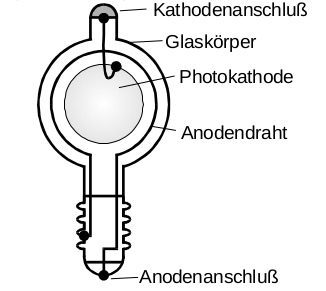
\includegraphics[height=5cm]{pictures/photozelle.png}
	\caption{Schematische Darstellung der verwendeten Photozelle \cite{anleitung}.}
	\label{fig:photozelle}
\end{figure}
\\
Für den Versuch wird ein optischer Aufbau, wie in \autoref{fig:OptischerAufbau}
dargestellt, verwendet. Das Licht einer Spektrallampe wird gebündelt und durch ein Prisma
räumlich in die einzelnen Spektrallinien aufgeteilt. Durch den Schwenkarm kann die
Spektrallinie und damit die Frequenz des Lichts ausgewählt werden, was aber immer
monochromatisch ist.
\begin{figure}
	\centering
	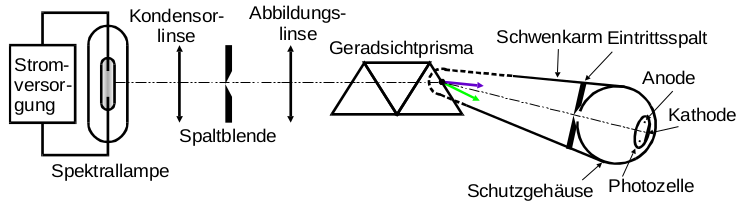
\includegraphics[height=5cm]{pictures/OptischerAufbau.png}
	\caption{Optischer Teil des Versuchsaufbaus \cite{anleitung}.}
	\label{fig:OptischerAufbau}
\end{figure}

\subsection{Energiemessung mit der Gegenfeldmethode}
\label{sec:Energiemessung mit der Gegenfeldmethode}

Um die Energie der einzelnen Photoelektronen zu bestimmen, wird hier mit der
Gegenfeldmethode gearbeitet. Dazu wird zwischen den Elektroden eine Spannung $U$ angelegt,
um ein abbremsendes Feld zu ergeugen. Der trotz jenem Feld fließende Strom zwischen Den
Elektroden wird mit einem Picoamperemeter gemessen. Der elektrische Aufbau ist in
\autoref{fig:ElektrischerAufbau} gezeigt.
\begin{figure}
	\centering
	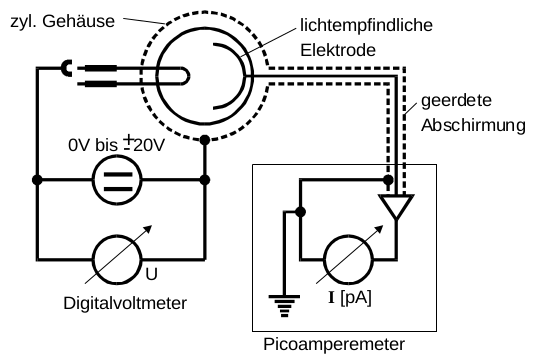
\includegraphics[height=6cm]{pictures/ElektrischerAufbau.png}
	\caption{Elektrisches Schaltbild der Messaparatur \cite{anleitung}.}
	\label{fig:ElektrischerAufbau}
\end{figure}
\\
Die Elektronen müssen nun auch das Potential des E-Feldes überwinden, aus der
Energieerhaltung folgt, dass der Strom verschwindet, wenn
\begin{equation}
	\label{eqn:v_max}
	e_0 U_\text{g} = \frac12 m_0 v_\text{max}^2,
\end{equation}
mit $v_\text{max}$ für die Geschwindigkeit der schnellsten Elektronen. 
Zusammen mit \autoref{eqn:theo:energiegleichung}
folgt 
\begin{equation}
	h\nu = e_0 U_\text{g} + A_\text{k}.
\end{equation}
Aus den Ergebnissen einer Messreihe ``Bremsspannung $U$ in Abhängigkeit von $\nu$`` lässt
sich dann das Verhältnis $\frac{h}{e_0}$ bestimmen.

\subsection{Fehlerquelle: Fermi-Dirac-Statistik}
\label{sec:Fehlerquelle: Fermi-Dirac-Statistik}

Ein großes Problem bei der in \autoref{sec:Energiemessung mit der Gegenfeldmethode}
beschriebenen Methode ist, dass der Photostrom nicht bei einer bestimmten Gegenspannung
$U_\text{g}$ verschwindet, sondern schon vorher ($U < U_\text{g}$) stark sinkt. Der
tatsächliche Verlauf $I(U)$ entspricht qualitativ dem in \autoref{fig:photostrom-approx}
gezeigten.
\\
Grund für dieses Verhalten ist, dass die Elektronen vor Ausstoßung verschiedene Energien
besitzen, die sich im Intervall von $0$ bis $\frac12 m_0 v_\text{max}^2$ befinden. Die
Energie der Photoelektronen hängt dann davon ab, welche Energie sie vorher im Festkörper
besessen haben. Diese Energieverteilung wird durch die Fermi-Dirac-Statistik beschrieben.
Nach dieser Statistik haben die außen liegenden Elektronen eine Energie zwischen $0$ und
der Fermi-Energie $\zeta$, eine geringe Anzahl kann sogar noch mehr Energie haben. Damit
lässt sich auch zeigen, dass unter bestimmten Vorrausetzungen ein parabolischer
Zusammenhang
\[
	I_\text{Ph} \sim U^2
\]
zwischen Photostrom und Bremsspannung $U$ besteht.

\begin{figure}
	\centering
	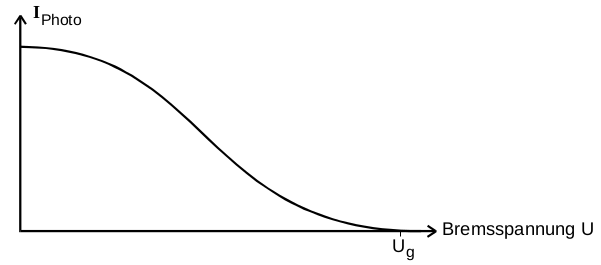
\includegraphics[height=5cm]{pictures/photostrom.png}
	\caption{Photostrom in Abhängigkeit von der Bremsspannung in einer mit monochromatischem Licht
	bestrahlten Photozelle \cite{anleitung}.}
	\label{fig:photostrom-approx}
\end{figure}

\subsection{Fehlerquelle: Hohe Austittsarbeit der Anode}
\label{sec:Fehlerquelle: Hohe Austittsarbeit der Anode}

Durch eine hohe Austrittsarbeit $A_\text{A}$ an der Anode kann ein Auftreten des Photostroms erschwert
werden. Gilt $A_\text{K} < h\nu < A_\text{A}$, so würde nach der linken Ungleichung ein
Photostrom auftreten, wegen der rechten müssen die Elektronen aber gegen ein Gegenfeld
anlauf. In diesem Fall ist erst mit einer beschleunigenden Spannung $U_\text{b}$, sodass
\[
	h\nu + e_0 U_\text{b} \geq A_\text{A}
\]
erfüllt ist. Mit der Photozelle in diesem Versuch sind bei niedrigen Spannungen sogar
negative Photoströme möglich, die die Bestimmung von $U_\text{g}$ weiter erschweren.

